\subsection{Calorimeter System}
\label{sec:Det:Calo}

The ATLAS calorimeter system, shown in Figure \ref{Det:ATLASCalo}, is a combination of different sampling detectors that are required to contain and measure both electromagnetic (EM) and hadronic showers over a large $|\eta|$ region. 
The main ATLAS calorimeter system consists of an EM calorimeter and a hadronic calorimeter, each of which aims to contain and measure EM and hadronic showers, respectively. 
There are also two forward calorimeters, one at each end of the experiment, at larger $\eta{}$, which measure both EM and hadronic energy deposits.
Different detector technology is used depending on the required accuracy for physics measurements and the radiation levels expected in different regions.
The amount of material, in radiation lengths, is shown in Figure \ref{Det:RadLegnth} for the different components of the ATLAS calorimeter system. 


\begin{figure}
  \centering
  \includegraphics[width=0.9\textwidth]{figures/Detector/AtlasCalorimeter.jpg}
\caption[The ATLAS Calorimeter System]{
Schematic of the ATLAS calorimeter system.
Figure from \cite{ref:ATLASExp}.
\label{Det:ATLASCalo}
}
\end{figure}

\begin{figure}
  \centering
  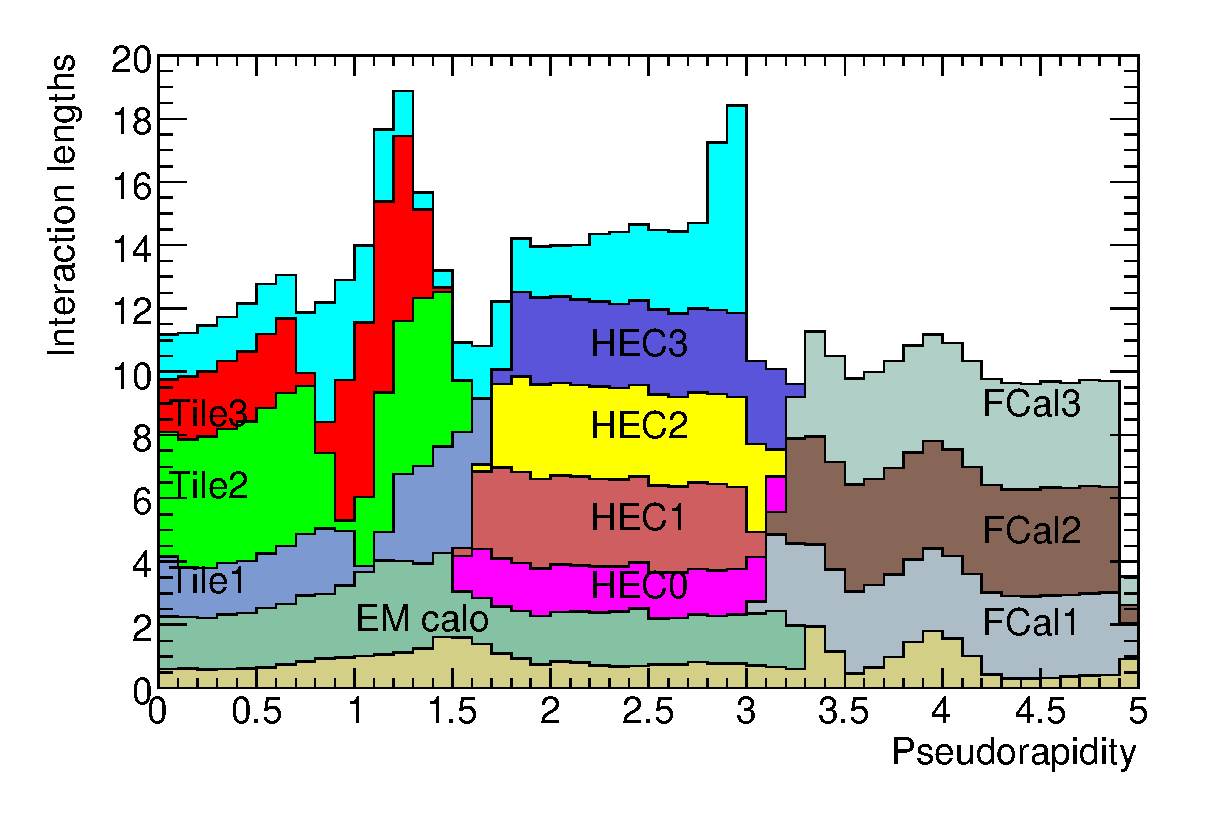
\includegraphics[width=0.9\textwidth]{figures/Detector/CalorimeterRadLegnths.eps}
  \caption[Radiation Lengths of the Calorimeter Sub-detectors ]{
Amount of material, in interaction lengths, in front of the different calorimeters.
The electromagnetic calorimeter is labelled ``EM calo'', the hadronic calorimeter is segmented into ``Tile'' and ``HEC'' layers, and the forward calorimeters is segmented with labels ``FCal''.
The final layer shown outermost for $|\eta|<3$ is the muon spectrometer.
Figure from \cite{ref:ATLASExp}.
\label{Det:RadLegnth}
}
\end{figure}





\subsubsection{EM Calorimeter}

The EM calorimeter is a sampling calorimeter with liquid argon (LAr) as the active material. 
It has complete azimuthal coverage for $|\eta|<3.2$ and is used to give precision measurements of EM showers.
Figure \ref{Det:ATLASCalo} shows the EM barrel and the EM end-cap, which have the pseudorapidity range $|\eta|<1.475$ and $1.375<|\eta|<3.2$, respectively.
In the precision region,  which is the region that overlaps the inner detector ($|\eta|<2.5$), there are three active layers and the detector is finely granulated to give a precise position measurement for the EM shower (used for photons).
Outside of the precision region there are two active layers and the granularity is coarser.
A presampler layer of LAr, which is in front of the first EM layer out to $|\eta|<1.8$, is used to correct for energy lost before the EM calorimeter. 
The EM calorimeter has greater than 22 radiation lengths to attempt to fully contain any EM showers.
The EM calorimeter cell information is calibrated to an EM scale using the decays of $Z$, $W$ and $\mathcal{J}/\psi$ as presented in \cite{ref:ZeeCalib}. 
The uncertainty on the electron EM scale is $<2\%$ for $|\eta|<2.7$ and $2-3\%$ for $2.5<|\eta|<4.9$. 

\subsubsection{Hadronic Calorimeter}



The hadronic calorimeter is situated behind the EM calorimeter covering the same $\eta$ region, and is responsible for the measurement of hadronic showers. 
It consists of three tile calorimeters (one barrel and two extended barrels) in the region $|\eta|<1.7$ and two hadronic end-caps (HEC) to extend the coverage to $|\eta|<3.2$ as shown in Figure \ref{Det:ATLASCalo}.
The hadronic calorimeter is a sampling detector, and the different components use different technologies with the tile calorimeter using  scintillating tiles as the active material and steel for the absorber, and the HECs using LAr as the active material and copper as the absorber.

The HEC has two wheels per end-cap, each with 32 wedged-shaped modules and has a granulation of $\Delta\eta~\rm{x}~\Delta\phi = 0.1~\rm{x}~0.1$ in the region $|\eta|<2.5$ and $\Delta\eta~\rm{x}~\Delta\phi = 0.2~\rm{x}~0.2$ in the region $2.5<|\eta|<3.2$.
Each wheel has two different depth segments, resulting in four layers per end-cap.

The tile calorimeter has three components, one barrel and two extended barrels.
The tile barrel and tile extended barrel cover the range $|\eta|<1$ and $0.8<|\eta|<1.7$ respectively.
These detectors comprise 64 modules which have a size of $\Delta\phi\approx0.1$, resulting in a granularity of $\Delta\eta~\rm{x}~\Delta\phi = 0.1~\rm{x}~0.1$.

\subsubsection{Forward Calorimeter}

The forward calorimeter (FCal), shown in Figure \ref{Det:ATLASCalo}, is responsible for measuring both the EM and hadronic showers in the region $3.2<|\eta|<4.9$.
The FCal has three detecting layers, the first layer is made of copper that is optimised for EM measurements and the following two are tungsten layers used to measure hadronic energy deposits.
All layers have LAr as the active material.
The choice of materials and design is largely determined by the need to be radiation hard to withstand the high particle flux.


\subsubsection{Calorimeter Objects}


To help construct offline physics objects, such as photons, electrons, taus or jets, an algorithm to cluster calorimeter readout cells is used.
The aim of clustering is to reconstruct the 3D EM or hadronic shower from the calorimeter cells.
Two clustering algorithms are used, the ``sliding window'' algorithm for photon, electron or tau identification, and the ``topological'' algorithm for jets.
The sliding window algorithm combines cell information from cells within a fixed size rectangular window in $\eta$ and $\phi$. 
Topological clusters, or ``topocluster'', are formed from a cluster seed, which is a cell with $|E|/\sigma_{noise}>4$, where $\sigma_{noise}$ is the expected noise in the calorimeter from the readout electronics and ``pile-up'' contributions. 
The cluster is then extended by including all cells next to it with $|E|/\sigma_{noise}>2$.
An additional layer of cells with $|E|/\sigma_{noise}>0$ are included.
The advantage of using this clustering rather than towers (groups of cells at fixed $\Delta\eta$ and $\Delta\phi$) is to improve noise suppression.
More information regarding topoclusters and sliding window clustering, and their performance, can be found in \cite{ref:ZeeCalib,ref:Clustering}.

%https://twiki.cern.ch/twiki/pub/Atlas/TapmJet/jetslice_v3_6April08.pdf

